\section{Последовательности максимального периода}
\selectlanguage{russian}
\label{section:max-seq}

Периодические последовательности с максимальным периодом называются $M$-последовательностями\index{$M$-последовательность} и характеризуются идеальной функцией автокорреляции.

Пусть $M$-последовательность имеет вид $x_1, x_2, \dots, x_n$, где значения $x_{i} = \pm 1$. Функция автокорреляции\index{функция!автокорреляции} такой последовательности имеет вид
\[
    \sum\limits_{i=1}^{T} x_i x_{i + \tau}  = \left\{ \begin{array}{l}
        -1, ~ \tau \neq 0, \\
        T, ~ \tau = 0. \\
    \end{array} \right.
\]

$M$-последовательности можно генерировать с помощью регистров сдвига с линейной обратной связью. На рис. \ref{fig:impulse} показан регистр сдвига, состоящий из ячеек памяти со входами для информационных символов и тактовых импульсов. На рис. \ref{fig:generator} тактовые импульсы опущены. Через $S_{j}$ обозначено содержимое $j$-й ячейки, где $j=\overline{0,L-1}$. В цепь обратной связи введены сумматоры по модулю 2 и умножители с коэффициентами $c_{j}$, принимающими значения $0,1$. Поступление тактового импульса вызывает сдвиг в регистре сдвига.
\begin{figure}[!ht]
	\centering
    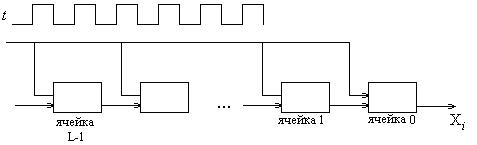
\includegraphics[width=0.8\textwidth]{pic/taktovi-impuls}
    \caption{Тактовые импульсы\label{fig:impulse}}
\end{figure}

В этой схеме используется линейная обратная связь. Выход ячейки с номером $L-1$ умножают на $c_{1}$, выход следующей ячейки $L-2$ умножают на $c_2$ и так далее. После умножения выходы ячеек суммируют по модулю 2 и результат подают на вход крайней ячейки $(L-1)$. Если содержимое всех ячеек состоит из нулей, то генерируемая последовательность также состоит из одних нулей. Если имеется ненулевое заполнение $S_{j-1}, S_{j-2}, \dots, S_{j-L}$, то после поступления $j$-го тактового импульса имеем сигнал на выходе такой, как показано на рис. \ref{fig:generator}:
\begin{figure}[!ht]
	\centering
	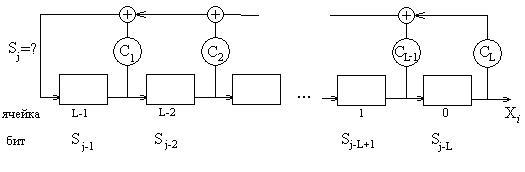
\includegraphics[width=0.8\textwidth]{pic/generator}
    \caption{Генератор\label{fig:generator}}
\end{figure}

Во всем разделе \ref{section:max-seq}  операцией <<$+$>>  обозначается операция сложения двоичных коэффициентов и многочленов по модулю 2.
\[
    S_{j} = c_{1} S_{j-1} + c_{2} S_{j-2} +  \dots  + c_{L-1} S_{j-L+1} + c_{L} S_{j-L}.
\]

Это соотношение определяет принцип работы генератора на регистрах сдвига\index{регистр сдвига}. Всего $2^{L}$ начальных условий, задающих значения бит в ячейках, из них $2^{L}-1$ ненулевых начальных условий. Генерируемая двоичная последовательность является периодической с периодом $T\leq 2^{L}-1$. Величина периода зависит от коэффициентов обратной связи $c_{1},  \ldots, c_{L} $.

Набор коэффициентов задается многочленом обратной связи
    \[ c(y) = 1 + c_1 y+ c_2 y^2 + \dots + c_L y^L. \]
Свойства этого многочлена влияют на период генерируемой последовательности. Рассмотрим его подробнее.

Многочлен $c(y)$ над полем $\GF{2}$ с коэффициентами $c_i \in \GF{2}$ называется \textit{приводимым}, если его можно представить в виде произведения многочленов меньшей степени. Например, многочлен $1 + y^{2} = (1 + y) (1 + y) = 1 + y + y + y^2 = 1 + y^2$ является приводимым. Многочлен $1 + y + y^{2}$ -- неприводимый.

Приведем без доказательства два важных утверждения.
\begin{itemize}
    \item Пусть $c(y)$ -- неприводимый многочлен. Тогда существует такое значение $m$, что $y^{m} + 1$ делится без остатка на $c(y)$, то есть $\frac{y^{m} + 1}{c(y)} = d(y)$.
    \item Существуют многочлены $c(y)$, для которых $m=2^{L} - 1$, где L -- степень многочлена $c(y)$. Эти многочлены называются примитивными.
\end{itemize}

Если $c(y)$ -- примитивный многочлен\index{многочлен!примитивный}, то период генерируемой последовательности является максимальным, то есть равным $T = 2^{L} - 1$. Генерируемые последовательности являются $M$-последовательностями, то есть последовательностями максимального периода. Для любого начального ненулевого состояния генерируется циклический сдвиг одной и той же последовательности максимального периода $T=2^{L} - 1$.

Оказывается, что многочлен обратной связи и состояние регистра определяются однозначно по $2L$ последовательным символам выхода регистра сдвига с линейной обратной связью (с помощью алгоритма Берлекэмпа~---~Мэсси или алгоритма Евклида).

Например, в спутниках GPS имеется регистр сдвига c 43 ячейками и периодом генерируемой последовательности $2^{43} - 1$. Длительность одного импульса $\sim 0{,}1$ мкс, период последовательности примерно равен одному году. Если бы для генерирования криптостойкой последовательности был просто применен регистр сдвига с линейной обратной связью, то, чтобы найти многочлен обратной связи, криптоаналитику достаточно было бы получить 86 символов последовательности.

Чтобы РСЛОС можно было использовать в качестве составной части криптографически стойкого генератора псевдослучайной последовательности или поточного шифра, создатели криптографических примитивов комбинируют несколько регистров сдвига, в том числе с помощью приводимых далее способов.
